% Created by tikzDevice version 0.12.3 on 2020-01-21 14:48:17
% !TEX encoding = UTF-8 Unicode
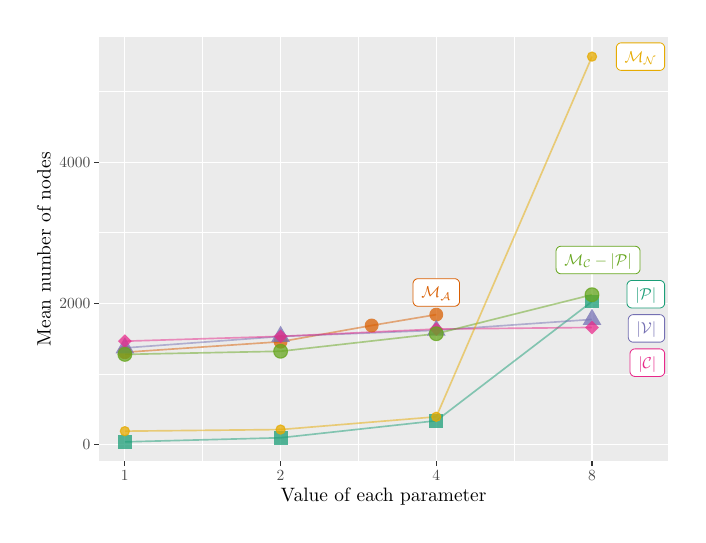
\begin{tikzpicture}[x=1pt,y=1pt]
\definecolor{fillColor}{RGB}{255,255,255}
\path[use as bounding box,fill=fillColor,fill opacity=0.00] (0,0) rectangle (234.88,176.16);
\begin{scope}
\path[clip] (  0.00,  0.00) rectangle (234.88,176.16);
\definecolor{drawColor}{RGB}{255,255,255}
\definecolor{fillColor}{RGB}{255,255,255}

\path[draw=drawColor,line width= 0.4pt,line join=round,line cap=round,fill=fillColor] (  0.00,  0.00) rectangle (234.88,176.16);
\end{scope}
\begin{scope}
\path[clip] ( 25.78, 19.53) rectangle (231.38,172.66);
\definecolor{fillColor}{gray}{0.92}

\path[fill=fillColor] ( 25.78, 19.53) rectangle (231.38,172.66);
\definecolor{drawColor}{RGB}{255,255,255}

\path[draw=drawColor,line width= 0.2pt,line join=round] ( 25.78, 51.08) --
	(231.38, 51.08);

\path[draw=drawColor,line width= 0.2pt,line join=round] ( 25.78,102.07) --
	(231.38,102.07);

\path[draw=drawColor,line width= 0.2pt,line join=round] ( 25.78,153.07) --
	(231.38,153.07);

\path[draw=drawColor,line width= 0.2pt,line join=round] ( 63.26, 19.53) --
	( 63.26,172.66);

\path[draw=drawColor,line width= 0.2pt,line join=round] (119.52, 19.53) --
	(119.52,172.66);

\path[draw=drawColor,line width= 0.2pt,line join=round] (175.79, 19.53) --
	(175.79,172.66);

\path[draw=drawColor,line width= 0.4pt,line join=round] ( 25.78, 25.58) --
	(231.38, 25.58);

\path[draw=drawColor,line width= 0.4pt,line join=round] ( 25.78, 76.58) --
	(231.38, 76.58);

\path[draw=drawColor,line width= 0.4pt,line join=round] ( 25.78,127.57) --
	(231.38,127.57);

\path[draw=drawColor,line width= 0.4pt,line join=round] ( 35.12, 19.53) --
	( 35.12,172.66);

\path[draw=drawColor,line width= 0.4pt,line join=round] ( 91.39, 19.53) --
	( 91.39,172.66);

\path[draw=drawColor,line width= 0.4pt,line join=round] (147.65, 19.53) --
	(147.65,172.66);

\path[draw=drawColor,line width= 0.4pt,line join=round] (203.92, 19.53) --
	(203.92,172.66);
\definecolor{drawColor}{RGB}{27,158,119}

\path[draw=drawColor,draw opacity=0.50,line width= 0.6pt,line join=round] ( 35.12, 26.49) --
	( 91.39, 27.97) --
	(147.65, 34.12) --
	(203.92, 77.20);
\definecolor{drawColor}{RGB}{217,95,2}

\path[draw=drawColor,draw opacity=0.50,line width= 0.6pt,line join=round] ( 35.12, 58.87) --
	( 91.39, 62.68) --
	(124.30, 68.55) --
	(147.65, 72.47);
\definecolor{drawColor}{RGB}{117,112,179}

\path[draw=drawColor,draw opacity=0.50,line width= 0.6pt,line join=round] ( 35.12, 60.44) --
	( 91.39, 64.58) --
	(147.65, 66.81) --
	(203.92, 70.73);
\definecolor{drawColor}{RGB}{231,41,138}

\path[draw=drawColor,draw opacity=0.50,line width= 0.6pt,line join=round] ( 35.12, 62.87) --
	( 91.39, 64.62) --
	(147.65, 67.25) --
	(203.92, 67.83);
\definecolor{drawColor}{RGB}{102,166,30}

\path[draw=drawColor,draw opacity=0.50,line width= 0.6pt,line join=round] ( 35.12, 58.10) --
	( 91.39, 59.23) --
	(147.65, 65.57) --
	(203.92, 79.66);
\definecolor{drawColor}{RGB}{230,171,2}

\path[draw=drawColor,draw opacity=0.50,line width= 0.6pt,line join=round] ( 35.12, 30.36) --
	( 91.39, 30.94) --
	(147.65, 35.55) --
	(203.92,165.70);
\definecolor{fillColor}{RGB}{27,158,119}

\path[fill=fillColor,fill opacity=0.75] ( 32.63, 23.99) --
	( 37.62, 23.99) --
	( 37.62, 28.99) --
	( 32.63, 28.99) --
	cycle;

\path[fill=fillColor,fill opacity=0.75] ( 88.89, 25.47) --
	( 93.89, 25.47) --
	( 93.89, 30.46) --
	( 88.89, 30.46) --
	cycle;

\path[fill=fillColor,fill opacity=0.75] (145.16, 31.63) --
	(150.15, 31.63) --
	(150.15, 36.62) --
	(145.16, 36.62) --
	cycle;

\path[fill=fillColor,fill opacity=0.75] (201.42, 74.70) --
	(206.42, 74.70) --
	(206.42, 79.69) --
	(201.42, 79.69) --
	cycle;
\definecolor{fillColor}{RGB}{217,95,2}

\path[fill=fillColor,fill opacity=0.75] ( 35.12, 58.87) circle (  2.50);

\path[fill=fillColor,fill opacity=0.75] ( 91.39, 62.68) circle (  2.50);

\path[fill=fillColor,fill opacity=0.75] (124.30, 68.55) circle (  2.50);

\path[fill=fillColor,fill opacity=0.75] (147.65, 72.47) circle (  2.50);
\definecolor{fillColor}{RGB}{117,112,179}

\path[fill=fillColor,fill opacity=0.75] ( 35.12, 64.32) --
	( 38.49, 58.50) --
	( 31.76, 58.50) --
	cycle;

\path[fill=fillColor,fill opacity=0.75] ( 91.39, 68.46) --
	( 94.75, 62.64) --
	( 88.03, 62.64) --
	cycle;

\path[fill=fillColor,fill opacity=0.75] (147.65, 70.70) --
	(151.02, 64.87) --
	(144.29, 64.87) --
	cycle;

\path[fill=fillColor,fill opacity=0.75] (203.92, 74.62) --
	(207.28, 68.79) --
	(200.56, 68.79) --
	cycle;
\definecolor{fillColor}{RGB}{231,41,138}

\path[fill=fillColor,fill opacity=0.75] ( 32.63, 62.87) --
	( 35.12, 65.37) --
	( 37.62, 62.87) --
	( 35.12, 60.37) --
	cycle;

\path[fill=fillColor,fill opacity=0.75] ( 88.89, 64.62) --
	( 91.39, 67.11) --
	( 93.89, 64.62) --
	( 91.39, 62.12) --
	cycle;

\path[fill=fillColor,fill opacity=0.75] (145.16, 67.25) --
	(147.65, 69.74) --
	(150.15, 67.25) --
	(147.65, 64.75) --
	cycle;

\path[fill=fillColor,fill opacity=0.75] (201.42, 67.83) --
	(203.92, 70.32) --
	(206.42, 67.83) --
	(203.92, 65.33) --
	cycle;
\definecolor{drawColor}{RGB}{102,166,30}
\definecolor{fillColor}{RGB}{102,166,30}

\path[draw=drawColor,draw opacity=0.75,line width= 0.4pt,line join=round,line cap=round,fill=fillColor,fill opacity=0.75] ( 35.12, 58.10) circle (  2.50);

\path[draw=drawColor,draw opacity=0.75,line width= 0.4pt,line join=round,line cap=round,fill=fillColor,fill opacity=0.75] ( 91.39, 59.23) circle (  2.50);

\path[draw=drawColor,draw opacity=0.75,line width= 0.4pt,line join=round,line cap=round,fill=fillColor,fill opacity=0.75] (147.65, 65.57) circle (  2.50);

\path[draw=drawColor,draw opacity=0.75,line width= 0.4pt,line join=round,line cap=round,fill=fillColor,fill opacity=0.75] (203.92, 79.66) circle (  2.50);
\definecolor{drawColor}{RGB}{230,171,2}
\definecolor{fillColor}{RGB}{230,171,2}

\path[draw=drawColor,draw opacity=0.75,line width= 0.4pt,line join=round,line cap=round,fill=fillColor,fill opacity=0.75] ( 35.12, 30.36) circle (  1.67);

\path[draw=drawColor,draw opacity=0.75,line width= 0.4pt,line join=round,line cap=round,fill=fillColor,fill opacity=0.75] ( 91.39, 30.94) circle (  1.67);

\path[draw=drawColor,draw opacity=0.75,line width= 0.4pt,line join=round,line cap=round,fill=fillColor,fill opacity=0.75] (147.65, 35.55) circle (  1.67);

\path[draw=drawColor,draw opacity=0.75,line width= 0.4pt,line join=round,line cap=round,fill=fillColor,fill opacity=0.75] (203.92,165.70) circle (  1.67);
\end{scope}
\begin{scope}
\path[clip] ( 25.78, 19.53) rectangle (231.38,172.66);

\path[] (216.56, 79.75) -- (203.92, 77.20);
\definecolor{drawColor}{RGB}{27,158,119}
\definecolor{fillColor}{RGB}{255,255,255}

\path[draw=drawColor,line width= 0.3pt,line join=round,line cap=round,fill=fillColor] (218.37, 74.87) --
	(228.37, 74.87) --
	(228.29, 74.88) --
	(228.58, 74.89) --
	(228.87, 74.94) --
	(229.14, 75.05) --
	(229.39, 75.19) --
	(229.62, 75.38) --
	(229.81, 75.60) --
	(229.97, 75.84) --
	(230.08, 76.11) --
	(230.15, 76.39) --
	(230.17, 76.68) --
	(230.17, 76.68) --
	(230.17, 83.01) --
	(230.17, 83.01) --
	(230.15, 83.30) --
	(230.08, 83.58) --
	(229.97, 83.85) --
	(229.81, 84.09) --
	(229.62, 84.31) --
	(229.39, 84.50) --
	(229.14, 84.64) --
	(228.87, 84.74) --
	(228.58, 84.80) --
	(228.37, 84.82) --
	(218.37, 84.82) --
	(218.59, 84.80) --
	(218.30, 84.81) --
	(218.01, 84.78) --
	(217.73, 84.70) --
	(217.47, 84.57) --
	(217.23, 84.41) --
	(217.02, 84.21) --
	(216.84, 83.97) --
	(216.71, 83.72) --
	(216.61, 83.44) --
	(216.57, 83.15) --
	(216.56, 83.01) --
	(216.56, 76.68) --
	(216.57, 76.83) --
	(216.57, 76.54) --
	(216.61, 76.25) --
	(216.71, 75.97) --
	(216.84, 75.71) --
	(217.02, 75.48) --
	(217.23, 75.28) --
	(217.47, 75.12) --
	(217.73, 74.99) --
	(218.01, 74.91) --
	(218.30, 74.88) --
	cycle;
\end{scope}
\begin{scope}
\path[clip] ( 25.78, 19.53) rectangle (231.38,172.66);
\definecolor{drawColor}{RGB}{27,158,119}

\node[text=drawColor,anchor=base,inner sep=0pt, outer sep=0pt, scale=  0.57] at (223.37, 77.88) {$|\mathcal{P}|$};
\end{scope}
\begin{scope}
\path[clip] ( 25.78, 19.53) rectangle (231.38,172.66);

\path[] (217.03, 67.65) -- (203.92, 70.73);
\definecolor{drawColor}{RGB}{117,112,179}
\definecolor{fillColor}{RGB}{255,255,255}

\path[draw=drawColor,line width= 0.3pt,line join=round,line cap=round,fill=fillColor] (218.84, 62.52) --
	(228.37, 62.52) --
	(228.29, 62.52) --
	(228.58, 62.53) --
	(228.87, 62.59) --
	(229.14, 62.69) --
	(229.39, 62.84) --
	(229.62, 63.02) --
	(229.81, 63.24) --
	(229.97, 63.48) --
	(230.08, 63.75) --
	(230.15, 64.03) --
	(230.17, 64.32) --
	(230.17, 64.32) --
	(230.17, 70.65) --
	(230.17, 70.65) --
	(230.15, 70.94) --
	(230.08, 71.22) --
	(229.97, 71.49) --
	(229.81, 71.74) --
	(229.62, 71.95) --
	(229.39, 72.14) --
	(229.14, 72.28) --
	(228.87, 72.39) --
	(228.58, 72.44) --
	(228.37, 72.46) --
	(218.84, 72.46) --
	(219.06, 72.44) --
	(218.77, 72.46) --
	(218.48, 72.42) --
	(218.20, 72.34) --
	(217.94, 72.22) --
	(217.70, 72.05) --
	(217.49, 71.85) --
	(217.31, 71.62) --
	(217.18, 71.36) --
	(217.09, 71.08) --
	(217.04, 70.80) --
	(217.03, 70.65) --
	(217.03, 64.32) --
	(217.04, 64.47) --
	(217.04, 64.18) --
	(217.09, 63.89) --
	(217.18, 63.61) --
	(217.31, 63.36) --
	(217.49, 63.12) --
	(217.70, 62.92) --
	(217.94, 62.76) --
	(218.20, 62.63) --
	(218.48, 62.55) --
	(218.77, 62.52) --
	cycle;
\end{scope}
\begin{scope}
\path[clip] ( 25.78, 19.53) rectangle (231.38,172.66);
\definecolor{drawColor}{RGB}{117,112,179}

\node[text=drawColor,anchor=base,inner sep=0pt, outer sep=0pt, scale=  0.57] at (223.60, 65.53) {$|\mathcal{V}|$};
\end{scope}
\begin{scope}
\path[clip] ( 25.78, 19.53) rectangle (231.38,172.66);

\path[] (217.66, 56.17) -- (203.92, 67.83);
\definecolor{drawColor}{RGB}{231,41,138}
\definecolor{fillColor}{RGB}{255,255,255}

\path[draw=drawColor,line width= 0.3pt,line join=round,line cap=round,fill=fillColor] (219.47, 50.14) --
	(228.37, 50.14) --
	(228.29, 50.14) --
	(228.58, 50.15) --
	(228.87, 50.21) --
	(229.14, 50.31) --
	(229.39, 50.46) --
	(229.62, 50.64) --
	(229.81, 50.86) --
	(229.97, 51.11) --
	(230.08, 51.37) --
	(230.15, 51.66) --
	(230.17, 51.95) --
	(230.17, 51.95) --
	(230.17, 58.27) --
	(230.17, 58.27) --
	(230.15, 58.56) --
	(230.08, 58.85) --
	(229.97, 59.11) --
	(229.81, 59.36) --
	(229.62, 59.58) --
	(229.39, 59.76) --
	(229.14, 59.91) --
	(228.87, 60.01) --
	(228.58, 60.07) --
	(228.37, 60.08) --
	(219.47, 60.08) --
	(219.68, 60.07) --
	(219.39, 60.08) --
	(219.11, 60.04) --
	(218.83, 59.96) --
	(218.56, 59.84) --
	(218.32, 59.67) --
	(218.11, 59.47) --
	(217.94, 59.24) --
	(217.80, 58.98) --
	(217.71, 58.71) --
	(217.67, 58.42) --
	(217.66, 58.27) --
	(217.66, 51.95) --
	(217.67, 52.09) --
	(217.67, 51.80) --
	(217.71, 51.51) --
	(217.80, 51.24) --
	(217.94, 50.98) --
	(218.11, 50.75) --
	(218.32, 50.55) --
	(218.56, 50.38) --
	(218.83, 50.26) --
	(219.11, 50.18) --
	(219.39, 50.14) --
	cycle;
\end{scope}
\begin{scope}
\path[clip] ( 25.78, 19.53) rectangle (231.38,172.66);
\definecolor{drawColor}{RGB}{231,41,138}

\node[text=drawColor,anchor=base,inner sep=0pt, outer sep=0pt, scale=  0.57] at (223.92, 53.15) {$|\mathcal{C}|$};
\end{scope}
\begin{scope}
\path[clip] ( 25.78, 19.53) rectangle (231.38,172.66);

\path[] (206.06, 87.23) -- (203.92, 79.66);
\definecolor{drawColor}{RGB}{102,166,30}
\definecolor{fillColor}{RGB}{255,255,255}

\path[draw=drawColor,line width= 0.3pt,line join=round,line cap=round,fill=fillColor] (192.74, 87.23) --
	(219.48, 87.23) --
	(219.40, 87.23) --
	(219.70, 87.24) --
	(219.98, 87.30) --
	(220.25, 87.40) --
	(220.50, 87.54) --
	(220.73, 87.73) --
	(220.92, 87.95) --
	(221.08, 88.19) --
	(221.19, 88.46) --
	(221.26, 88.74) --
	(221.28, 89.03) --
	(221.28, 89.03) --
	(221.28, 95.36) --
	(221.28, 95.36) --
	(221.26, 95.65) --
	(221.19, 95.93) --
	(221.08, 96.20) --
	(220.92, 96.45) --
	(220.73, 96.66) --
	(220.50, 96.85) --
	(220.25, 96.99) --
	(219.98, 97.10) --
	(219.70, 97.15) --
	(219.48, 97.17) --
	(192.74, 97.17) --
	(192.95, 97.15) --
	(192.66, 97.17) --
	(192.37, 97.13) --
	(192.10, 97.05) --
	(191.83, 96.93) --
	(191.59, 96.76) --
	(191.38, 96.56) --
	(191.21, 96.33) --
	(191.07, 96.07) --
	(190.98, 95.79) --
	(190.94, 95.51) --
	(190.93, 95.36) --
	(190.93, 89.03) --
	(190.94, 89.18) --
	(190.94, 88.89) --
	(190.98, 88.60) --
	(191.07, 88.32) --
	(191.21, 88.07) --
	(191.38, 87.83) --
	(191.59, 87.63) --
	(191.83, 87.47) --
	(192.10, 87.34) --
	(192.37, 87.26) --
	(192.66, 87.23) --
	cycle;
\end{scope}
\begin{scope}
\path[clip] ( 25.78, 19.53) rectangle (231.38,172.66);
\definecolor{drawColor}{RGB}{102,166,30}

\node[text=drawColor,anchor=base,inner sep=0pt, outer sep=0pt, scale=  0.57] at (206.11, 90.24) {$\mathcal{M}_{\mathcal{C}}-|\mathcal{P}|$};
\end{scope}
\begin{scope}
\path[clip] ( 25.78, 19.53) rectangle (231.38,172.66);

\path[] (212.71,165.70) -- (203.92,165.70);
\definecolor{drawColor}{RGB}{230,171,2}
\definecolor{fillColor}{RGB}{255,255,255}

\path[draw=drawColor,line width= 0.3pt,line join=round,line cap=round,fill=fillColor] (214.51,160.73) --
	(228.37,160.73) --
	(228.29,160.73) --
	(228.58,160.74) --
	(228.87,160.80) --
	(229.14,160.90) --
	(229.39,161.05) --
	(229.62,161.23) --
	(229.81,161.45) --
	(229.97,161.69) --
	(230.08,161.96) --
	(230.15,162.24) --
	(230.17,162.53) --
	(230.17,162.53) --
	(230.17,168.86) --
	(230.17,168.86) --
	(230.15,169.15) --
	(230.08,169.43) --
	(229.97,169.70) --
	(229.81,169.95) --
	(229.62,170.16) --
	(229.39,170.35) --
	(229.14,170.49) --
	(228.87,170.60) --
	(228.58,170.66) --
	(228.37,170.67) --
	(214.51,170.67) --
	(214.73,170.66) --
	(214.44,170.67) --
	(214.15,170.63) --
	(213.87,170.55) --
	(213.61,170.43) --
	(213.37,170.26) --
	(213.16,170.06) --
	(212.99,169.83) --
	(212.85,169.57) --
	(212.76,169.29) --
	(212.71,169.01) --
	(212.71,168.86) --
	(212.71,162.53) --
	(212.71,162.68) --
	(212.71,162.39) --
	(212.76,162.10) --
	(212.85,161.82) --
	(212.99,161.57) --
	(213.16,161.34) --
	(213.37,161.13) --
	(213.61,160.97) --
	(213.87,160.84) --
	(214.15,160.76) --
	(214.44,160.73) --
	cycle;
\end{scope}
\begin{scope}
\path[clip] ( 25.78, 19.53) rectangle (231.38,172.66);
\definecolor{drawColor}{RGB}{230,171,2}

\node[text=drawColor,anchor=base,inner sep=0pt, outer sep=0pt, scale=  0.57] at (221.44,163.74) {$\mathcal{M}_{\mathcal{N}}$};
\end{scope}
\begin{scope}
\path[clip] ( 25.78, 19.53) rectangle (231.38,172.66);
\definecolor{drawColor}{RGB}{217,95,2}
\definecolor{fillColor}{RGB}{255,255,255}

\path[draw=drawColor,line width= 0.3pt,line join=round,line cap=round,fill=fillColor] (141.06, 75.50) --
	(154.25, 75.50) --
	(154.17, 75.51) --
	(154.46, 75.52) --
	(154.75, 75.58) --
	(155.02, 75.68) --
	(155.27, 75.82) --
	(155.50, 76.01) --
	(155.69, 76.23) --
	(155.85, 76.47) --
	(155.96, 76.74) --
	(156.03, 77.02) --
	(156.05, 77.31) --
	(156.05, 77.31) --
	(156.05, 83.64) --
	(156.05, 83.64) --
	(156.03, 83.93) --
	(155.96, 84.21) --
	(155.85, 84.48) --
	(155.69, 84.73) --
	(155.50, 84.94) --
	(155.27, 85.13) --
	(155.02, 85.27) --
	(154.75, 85.38) --
	(154.46, 85.43) --
	(154.25, 85.45) --
	(141.06, 85.45) --
	(141.28, 85.43) --
	(140.99, 85.44) --
	(140.70, 85.41) --
	(140.42, 85.33) --
	(140.16, 85.20) --
	(139.92, 85.04) --
	(139.71, 84.84) --
	(139.54, 84.61) --
	(139.40, 84.35) --
	(139.31, 84.07) --
	(139.26, 83.79) --
	(139.26, 83.64) --
	(139.26, 77.31) --
	(139.26, 77.46) --
	(139.26, 77.17) --
	(139.31, 76.88) --
	(139.40, 76.60) --
	(139.54, 76.35) --
	(139.71, 76.11) --
	(139.92, 75.91) --
	(140.16, 75.75) --
	(140.42, 75.62) --
	(140.70, 75.54) --
	(140.99, 75.51) --
	cycle;
\end{scope}
\begin{scope}
\path[clip] ( 25.78, 19.53) rectangle (231.38,172.66);
\definecolor{drawColor}{RGB}{217,95,2}

\node[text=drawColor,anchor=base,inner sep=0pt, outer sep=0pt, scale=  0.57] at (147.65, 78.52) {$\mathcal{M}_{\mathcal{A}}$};
\end{scope}
\begin{scope}
\path[clip] (  0.00,  0.00) rectangle (234.88,176.16);
\definecolor{drawColor}{gray}{0.30}

\node[text=drawColor,anchor=base east,inner sep=0pt, outer sep=0pt, scale=  0.56] at ( 22.63, 23.65) {0};

\node[text=drawColor,anchor=base east,inner sep=0pt, outer sep=0pt, scale=  0.56] at ( 22.63, 74.65) {2000};

\node[text=drawColor,anchor=base east,inner sep=0pt, outer sep=0pt, scale=  0.56] at ( 22.63,125.64) {4000};
\end{scope}
\begin{scope}
\path[clip] (  0.00,  0.00) rectangle (234.88,176.16);
\definecolor{drawColor}{gray}{0.20}

\path[draw=drawColor,line width= 0.4pt,line join=round] ( 24.03, 25.58) --
	( 25.78, 25.58);

\path[draw=drawColor,line width= 0.4pt,line join=round] ( 24.03, 76.58) --
	( 25.78, 76.58);

\path[draw=drawColor,line width= 0.4pt,line join=round] ( 24.03,127.57) --
	( 25.78,127.57);
\end{scope}
\begin{scope}
\path[clip] (  0.00,  0.00) rectangle (234.88,176.16);
\definecolor{drawColor}{gray}{0.20}

\path[draw=drawColor,line width= 0.4pt,line join=round] ( 35.12, 17.78) --
	( 35.12, 19.53);

\path[draw=drawColor,line width= 0.4pt,line join=round] ( 91.39, 17.78) --
	( 91.39, 19.53);

\path[draw=drawColor,line width= 0.4pt,line join=round] (147.65, 17.78) --
	(147.65, 19.53);

\path[draw=drawColor,line width= 0.4pt,line join=round] (203.92, 17.78) --
	(203.92, 19.53);
\end{scope}
\begin{scope}
\path[clip] (  0.00,  0.00) rectangle (234.88,176.16);
\definecolor{drawColor}{gray}{0.30}

\node[text=drawColor,anchor=base,inner sep=0pt, outer sep=0pt, scale=  0.56] at ( 35.12, 12.52) {1};

\node[text=drawColor,anchor=base,inner sep=0pt, outer sep=0pt, scale=  0.56] at ( 91.39, 12.52) {2};

\node[text=drawColor,anchor=base,inner sep=0pt, outer sep=0pt, scale=  0.56] at (147.65, 12.52) {4};

\node[text=drawColor,anchor=base,inner sep=0pt, outer sep=0pt, scale=  0.56] at (203.92, 12.52) {8};
\end{scope}
\begin{scope}
\path[clip] (  0.00,  0.00) rectangle (234.88,176.16);
\definecolor{drawColor}{RGB}{0,0,0}

\node[text=drawColor,anchor=base,inner sep=0pt, outer sep=0pt, scale=  0.70] at (128.58,  4.86) {Value of each parameter};
\end{scope}
\begin{scope}
\path[clip] (  0.00,  0.00) rectangle (234.88,176.16);
\definecolor{drawColor}{RGB}{0,0,0}

\node[text=drawColor,rotate= 90.00,anchor=base,inner sep=0pt, outer sep=0pt, scale=  0.70] at (  8.32, 96.09) {Mean number of nodes};
\end{scope}
\end{tikzpicture}
